\documentclass[12pt,a4paper,bibliography=totoc,listof=totoc]{scrartcl}
% u.U. muss Koma-Skript Package ueber MikTeX deinstalliert und neu installiert werden
% Hilft das nicht, so sollte statt scrartcl die Dokumentenklasse article verwendet werden
\usepackage[ngerman]{babel}
\usepackage[utf8]{inputenc}
\usepackage{ifthen}
\usepackage{xargs}
\usepackage{amsmath}
\usepackage{amsfonts}
\usepackage{amssymb}
\usepackage{graphicx}
\usepackage{fancyhdr}
\usepackage{tabularx}
\usepackage{geometry}
\usepackage{setspace}
\usepackage[right]{eurosym}
\usepackage[printonlyused]{acronym}
\usepackage{subfig}
\usepackage{floatflt}
\usepackage{float}
\usepackage[usenames,dvipsnames]{color}
\usepackage{colortbl}
\usepackage{paralist}
\usepackage{array}
\usepackage{parskip}
\usepackage[right]{eurosym}
\usepackage[subfigure,titles]{tocloft}
\usepackage[pdfpagelabels=true]{hyperref}

\usepackage{listings}
\lstset{basicstyle=\footnotesize, captionpos=b, breaklines=true, showstringspaces=false, tabsize=2, frame=lines, numbers=left, numberstyle=\tiny, xleftmargin=2em, framexleftmargin=2em}
\makeatletter
\def\l@lstlisting#1#2{\@dottedtocline{1}{0em}{1em}{\hspace{1,5em} Lst. #1}{#2}}
\makeatother

\geometry{a4paper, top=35mm, left=35mm, right=25mm, bottom=40mm, headsep=10mm, footskip=10mm}

\definecolor{codered}{rgb}{0.6,0,0} % for strings
\definecolor{codegreen}{rgb}{0.25,0.5,0.35} % comments
\definecolor{codepurple}{rgb}{0.5,0,0.35} % keywords
\definecolor{codeblue}{rgb}{0.25,0.35,0.75} 
\definecolor{codegray}{rgb}{0.6,0.6,0.6}
 
\lstset{language=C,
basicstyle=\ttfamily\footnotesize,
keywordstyle=\color{codepurple}\bfseries,
stringstyle=\color{codered},
commentstyle=\color{codegreen}\itshape\bfseries,
morecomment=[s][\color{codeblue}]{/**}{*/},
numbers=left,
numberstyle=\tiny\color{codegray},
stepnumber=1,
numbersep=10pt,
tabsize=2,
showspaces=false,
showstringspaces=false}


% begin change
%\titlespacing{\section}{0pt}{12pt plus 4pt minus 2pt}{-6pt plus 2pt minus 2pt}
% end change

% Kopf- und Fusszeile
\renewcommand{\sectionmark}[1]{\markright{#1}}
\renewcommand{\leftmark}{\rightmark}
\pagestyle{fancy}
\lhead{}
\chead{}
\rhead{\thesection\space\contentsname}
\lfoot{}
\cfoot{}
\rfoot{\ \linebreak \thepage}
\renewcommand{\headrulewidth}{0.4pt}
\renewcommand{\footrulewidth}{0.4pt}

% Vorspann
\renewcommand{\thesection}{\Roman{section}}
\renewcommand{\theHsection}{\Roman{section}}
\pagenumbering{Roman}

\newcommand{\folgen}[1]{
\ensuremath
#1
}

\newcommandx{\student}[3][]{
	\def\studentName{#1}%
	\def\studentMatnr{#2}%
	\def\studentStudiengang{#3}%
}

\newcommandx{\studentt}[3][]{
	\def\studentNamet{#1}%
	\def\studentMatnrt{#2}%
	\def\studentStudiengangt{#3}%
}


\newcommandx{\studenttt}[3][]{
	\def\studentNamett{#1}%
	\def\studentMatnrtt{#2}%
	\def\studentStudiengangtt{#3}%
}


\newcommandx{\MyTitelseite}[8][]{
\thispagestyle{empty}
%
\includegraphics[scale=0.2]{pics/oth-logo.png}\hfill\includegraphics[scale=0.2]{#1}

\includegraphics[scale=0.2]{pics/oth-logo.png}
\begin{center}
\ifthenelse{\equal{#2}{2}}{ % then
	\vspace*{2cm}
	\Large
	\textbf{Ostbayerische Technische Hochschule Regensburg}\\
	\textbf{Fakultät für Informatik und Mathematik}\\
	\vspace*{2cm}
	\Huge
	\textbf{#3}\\[1em]
	\large
	%Zur Erlangung des akademischen Grades des\\
	%\ifthenelse{\equal{#3}{Bachelorarbeit}}{Bachelor of Science (B.Sc.)}{Master of Science (M.Sc.)}\\
	\vspace*{1cm}
	\Large
	\textbf{#4}\\
}{ % else
	\vspace*{1cm}
	\Large
	\textbf{#4}\\
	\vspace*{2cm}
	\large
	An der Fakultät für Informatik und Mathematik der\\
	Ostbayerischen Technischen Hochschule Regensburg\\
	im Studiengang\\
	\studentStudiengang\\[2em]
	eingereichte\\
	\vspace*{1cm}
	\Large
	\textbf{#3}\\[2em]
	\large
	%zur Erlangung des akademischen Grades des\\
	%\ifthenelse{\equal{#3}{Bachelorarbeit}}{Bachelor of Science (B.Sc.)}{Master of Science (M.Sc.)}
	\vspace*{1cm}
	\Large
}
	\vfill
	\normalsize
	%\newcolumntype{x}[1]{>{\raggedleft\arraybackslash\hspace{0pt}}p{#1}}
	\begin{tabular}{rl}%{6cm}p{7.5cm}}
	    \rule{0mm}{1ex}\textbf{Name:} & \studentName \\
		\rule{0mm}{1ex}\textbf{Matrikelnummer:} & \hspace*{-0.5em}\begin{tabular}[t]{r}\studentMatnr\end{tabular} \\ 
		\rule{0mm}{1ex}\textbf{Name:} & \studentNamet \\
		\rule{0mm}{1ex}\textbf{Matrikelnummer:} & \hspace*{-0.5em}\begin{tabular}[t]{r}\studentMatnrt\end{tabular} \\ 
		\rule{0mm}{1ex}\textbf{Name:} & \studentNamett \\
		\rule{0mm}{1ex}\textbf{Matrikelnummer:} & \hspace*{-0.5em}\begin{tabular}[t]{r}\studentMatnrtt\end{tabular} \\ 
		\ifthenelse{\equal{#2}{1}}{~\\}{\rule{0mm}{1ex}\textbf{Studiengang:} & \studentStudiengang \\[2em]}
		\rule{0mm}{1ex}\textbf{Erstgutachter:} & #5 \\ 
		%\rule{0mm}{1ex}\textbf{Zweitgutachter:} & #6 \\[2em]
		\rule{0mm}{1ex}\textbf{Abgabedatum:} & #7 \\
	\end{tabular} 
	

%\end{center}	
%\end{center}
	
	
\end{center}
\pagebreak
}

\begin{document}


% ----------------------------------------------------------------------------------------------------------
% Titelseite
% ----------------------------------------------------------------------------------------------------------
\student{Name des Studierenden}	% Studierender
{1234567}						% Matrikelnummer
{Technische Informatik}			% Studiengang

%\MyTitelseite{pics/oth-logo-informatik.png}	% Optionales Logo des extern betreuenden Unternehmens
\MyTitelseite{}
{1}								% Style der Titelseite (1 oder 2)
{Projektarbeit in DAFP(Angewandte FPGA Programmierung)}			% Typ der Arbeit 
{Thema der Arbeit}				% Thema der Arbeit						
{Prof.\ Dr.\ Name des Erstgutachters}   % Betreuer
{Prof.\ Dr.\ Name des Zweitgutachters}	% Zweitgutachter
{??.??.\the\year}				% Abgabedatum

\setcounter{page}{1} 

%-----------------------------------------------------------------------------------------------------------
% Abstract ZUsammenfassung
%-----------------------------------------------------------------------------------------------------------
%\section*{Kurzfassung}
%...
%\pagebreak

%\section*{Abstract}
%...
%\pagebreak

%\section*{Danksagung}
%...
%\pagebreak

% ----------------------------------------------------------------------------------------------------------
% Inhaltsverzeichnis
% ----------------------------------------------------------------------------------------------------------
\tableofcontents
\pagebreak
% ----------------------------------------------------------------------------------------------------------
% Inhalt
% ----------------------------------------------------------------------------------------------------------
% Abstände Überschrift
% begin change
% alte Befehle
%\titlespacing{\section}{0pt}{12pt plus 4pt minus 2pt}{-6pt plus 2pt minus 2pt}
%\titlespacing{\subsection}{0pt}{12pt plus 4pt minus 2pt}{-6pt plus 2pt minus 2pt}
%\titlespacing{\subsubsection}{0pt}{12pt plus 4pt minus 2pt}{-6pt plus 2pt minus 2pt}
% neue Befehle
\RedeclareSectionCommands[
beforeskip=-.9\baselineskip,
afterskip=.4\baselineskip
]{section,subsection,subsubsection}
%end change

% Kopfzeile
\renewcommand{\sectionmark}[1]{\markright{#1}}
\renewcommand{\subsectionmark}[1]{}
\renewcommand{\subsubsectionmark}[1]{}
\lhead{Kapitel \thesection}
\rhead{\rightmark}

%\onehalfspacing
\setstretch{1.15}
\renewcommand{\thesection}{\arabic{section}}
\renewcommand{\theHsection}{\arabic{section}}
\setcounter{section}{0}
\pagenumbering{arabic}
\setcounter{page}{1}

% ----------------------------------------------------------------------------------
% Kapitel: Einleitung
% ----------------------------------------------------------------------------------
\section{Einleitung}


\pagebreak
% ----------------------------------------------------------------------------------
% Kapitel: ???
% ----------------------------------------------------------------------------------
\section{Kapitel 3: Timing und Blank\_Check Korbinian Federholzner}
\subsection{Überblick}
Um Pixel auf dem Bildschirm setzen zu können, müssen zwei Signale an diesem anlegen. Diese sind unterteilt in ein horizontales und ein vertikales Signal. 
Da das Schreiben der Pixel auf dem Bildschirm von links nach rechts erfolgt, muss nachdem der letzte Pixel der Zeile gesetzt worden ist auf die erste Stelle 
der nächsten Zeile zurückgekehrt werden. In diesem Zeitraum muss kurz gewartet, sowie synchronisiert werden. Es darf auch wärend dessen kein Pixel an den Bildschirm
geschickt werden. Der "Blank Check" soll, dass verhindern, indem er die Pixel die, geschickt werden würden auf schwarz setzt. Da nicht immer der gleiche Pixel 
geschrieben werden soll muss an den Speicher eine Adresse, des Pixels für die jeweilige Position geschickt werden. 

\vspace{1em}
\begin{minipage}{\linewidth}
	\centering
	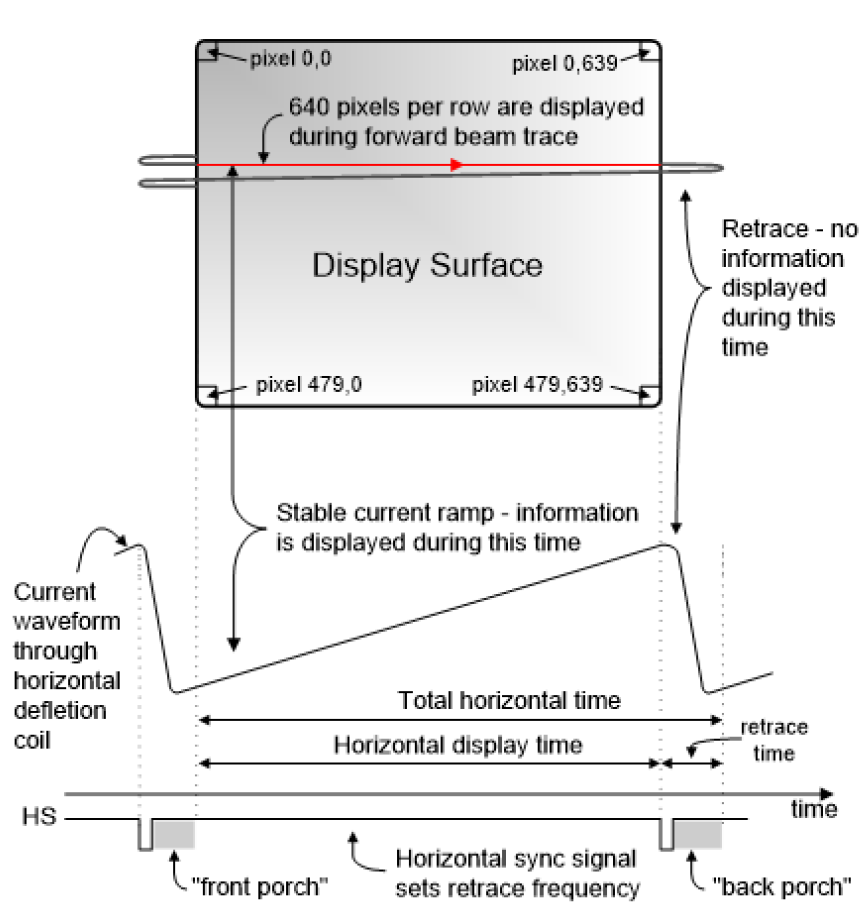
\includegraphics[width=0.8\linewidth]{pics/VGA_Erkl.png}
	\captionof{figure}[VGASchematic]{VGA Synchronisation}
	\label{fig:VGASchematic}
\end{minipage}

Hier sieht man, dass die Wartezeit vom Zurücksetzen zum Anfang durch eine Backporch, eine Frontporch und eine Synchronisation erfolgen.

\subsection{Lösungsätze}
Um das Timing der horizontalen und vertikalen Synchronisation Signale einhalten zu können, muss mindestens ein Zähler/Counter implementiert werden, welcher als Timer dient.
Ein weiterer Ansatz ist zwei Timer zu wählen, jeweils für die beiden Signale. Da auch die Position des Pixels and den Speicher geschickt werden soll, kann man diese 
beiden Timer als Andressen-Zugriff verwenden. Desweitern könnte man auch 2 Timer und 2 Zähler/Counter wählen, jeweils für das Einhalten der Zeiten und den Stand des momentan 
Pixels. 
Bei der Aufteilung in Prozessen, gibt es auch mehrere Möglichkeiten. Z.B. Aufteilung in drei Prozesse für Blank und die beiden Synchronisation Signale. Nun mehr diese 
abhängig vom Timer-Stand setzen. 
\vspace{1em}
\lstinputlisting[caption=Pseudo-Code 3 Prozesse, label=lst:threeProcesses,basicstyle=\ttfamily\scriptsize]{code/threeProcesses.vhd}
Der Prozess für Blank kann weggelassen werden und asynchron implementiert werden.
Auch möglich sind zwei Prozesse als Zustandsautomaten welche abhängig vom Stand der Timer sind und jeweils die drei Signale setzt.
\vspace{1em}
\lstinputlisting[caption=Pseudo-Code für den Zustandsautomaten, label=lst:Statemachine,basicstyle=\ttfamily\scriptsize]{code/Statemachine.vhd}
Man kann die Zustände auch ändern, indem diese abhängig macht wann sich die Signale (horizontal, vertikal und Blank) ändern, vergleiche \ref{lst:threeProcesses}
Die Timer/Zähler kommen jeweils als Prozesse oder Komponenten hinzu.
\newline
Der Ansatz mit den 2 Timern und 2 Zählern/Countern wird verwendet, da dadurch die Timer in der Komponente versteckt werden und nur die momentane Zeilen- und 
Spaltenposition der Counter ausgegeben wird. Bei den Porches sowie der Synchronisation werden diese auf 0 gesetzt (kein darüber hinauszählen keine
Speicherzugriffsfehler). Außerdem wird ein Zustandsautomat verwendet, siehe \ref{lst:Statemachine}, da es dieser leichter macht den Code in der Simulation
zu begutachten, sowie die Funktionen der Porches und Synchronisation-Signale im Code nachzuvollziehen.

\subsection{Implementierung}
Die beiden Timer benutzen die gleiche Komponente (Timer-Component). Die Zähler verwenden auch eine eigene (Counter-Component). Man könnte auch beide in eine Komponente 
zusammenfassen, jedoch wurden sie getrennt. Dies liegt daran, dass der Zähler nur manchmal läuft, und deswegen ein INC Signal braucht. Außerdem verwendet der Zähler den 
std\_logic\_vector und der Timer integer zur leichteren Überprüfung, durch die Trennung kann auf Typumwandlung verzichtet werden.
Die Abfrage der Timer auf die Zeiten zum Zustandswechsel, wird mithilfe einer Funktion zur Umwandlung von Nanosekunden in Taktzyklen vollbracht.
Als Code-Struktur wird eine Statemachine verwendet, siehe \ref{lst:Statemachine}. Mit 2 Prozessen, für das horizontale sowie das vertikale Signal. Das Blank wird in den
jeweiligen States gesetzt. Dadurch wird ein Signal an die Blank Komponente gesendet, welche jedes eingehende Signal vom Speicher auf 0 setzt (schwarz).

\subsection{Optimierung}
Es gibt den Asynchronen Reset und den Synchronen Reset, welche verglichen werden.
Das Zurücksetzen von Timern, Zählern, sowie States und Signalen, erfolgt in den jeweiligen Komponenten, die Sync-Gen Komponente hat für beide Prozesse einen Reset, um
Timern, Zählern, sowie States und Signalen zurückzusetzen. Die Timer und Zähler hingegen nur ein Reset Signal zum Zurücksetzen ihres Zählerswertes. Sind in allen 
Komponenten Synchrone Resets, so ergibt sich folgende Hardwarebelegung:

\vspace{1em}
\begin{minipage}{\linewidth}
	\centering
	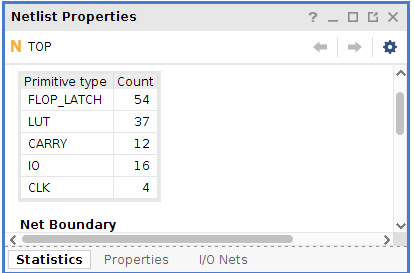
\includegraphics[width=0.5\linewidth]{pics/SynchronousNetListProperties.png}
	\captionof{figure}[SynchronReset]{Synchroner Reset}
	\label{fig:Synchroner Reset}
\end{minipage}

Im Gegensatz dazu falls ein Asynchronener Reset verwendet wird:

\vspace{1em}
\begin{minipage}{\linewidth}
	\centering
	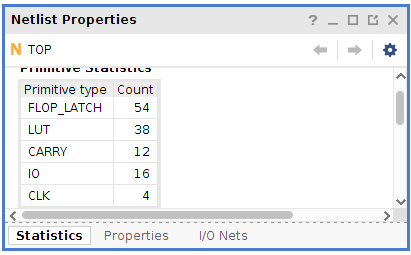
\includegraphics[width=0.5\linewidth]{pics/AsynchronousNetList.png}
	\captionof{figure}[AsynchronReset]{Asynchroner Reset}
	\label{fig: Asynchroner Reset}
\end{minipage}

vergleicht man nun von beiden den Hardwareaufbau

\vspace{1em}
\begin{minipage}{\linewidth}
	\centering
	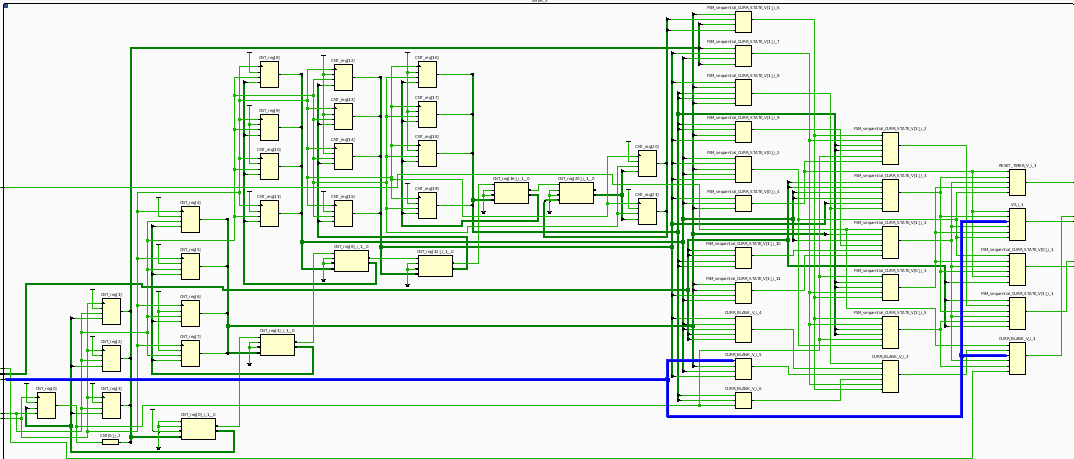
\includegraphics[width=1.0\linewidth]{pics/FullSchematicAsynchronusly.png}
	\captionof{figure}[AsynchronResetHW]{Hardware Generierung des Asynchroner Resets}
	\label{fig: Asynchroner Reset HW}
\end{minipage}


\vspace{1em}
\begin{minipage}{\linewidth}
	\centering
	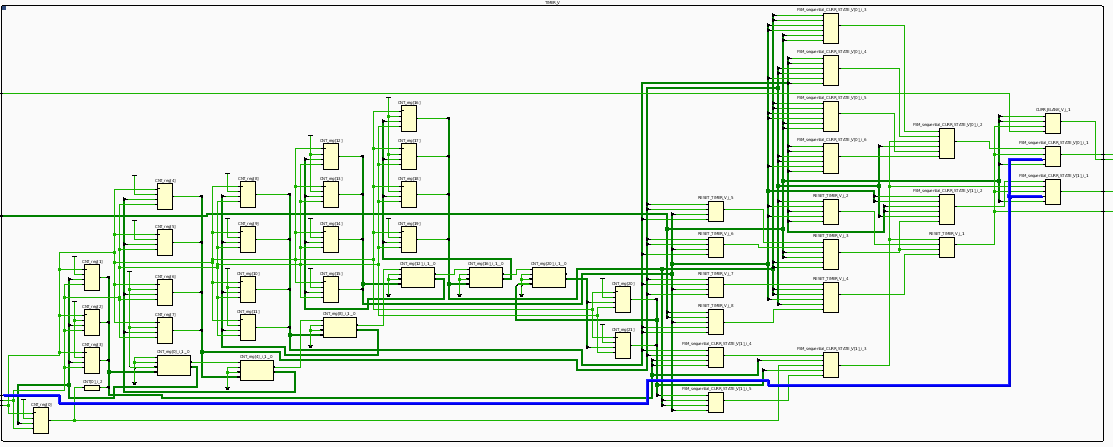
\includegraphics[width=1.0\linewidth]{pics/FullSchmeaticSyncronous.png}
	\captionof{figure}[AsynchronReset]{Hardware Generierung des Synchronen Resets}
	\label{fig:Synchroner Reset HW}
\end{minipage}

kann man erkennen, dass beim Asynchronen Reset ein weiterer Lookup Table generiert wird, welcher auch am Reset Signal angeschlossen ist.
\newline
Eine Weitere Optimierung ist, den Globalen Reset der Sync-Gen Komponente zu entfehrnen. Dies ist möglich, da falls der Speicher im Hintergrund
Zurücksetzt wird, einfach an der Stelle im Speicher an dem der Zähler im moment ist weitergelesen wird und danach wieder von vorne angefangen wird.
auf dem Bildschirm kann das Auge dann keinen Unterschied erkennen (eventuell ist der Erste Frame etwas falsch).

\vspace{1em}
\begin{minipage}{\linewidth}
	\centering
	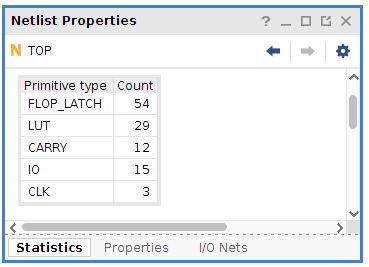
\includegraphics[width=0.5\linewidth]{pics/ohneResetNetProp.png}
	\captionof{figure}[noReset]{ohne Globalen Reset}
	\label{fig:no Reset}
\end{minipage}

Bei diesem Bild sieht man dass erneut Lookup Tables wegfallen. Die Resets der Timer und Zähler wurden nicht entfehrnt, da sie weiterhin zurückgesetzt werden 
sollen, falls ein Timer oder Zähler seinen Maximalwert erreicht.


\pagebreak
% ----------------------------------------------------------------------------------
% Kapitel: Fazit und Ausblick
% ----------------------------------------------------------------------------------
\section{Fazit und Ausblick}


\pagebreak
% ----------------------------------------------------------------------------------
% Kleine Einführung in LaTeX-Elemente
% ----------------------------------------------------------------------------------
\section{\LaTeX-Elemente}
Dieser Abschnitt beinhaltet lediglich einige Informationen über \LaTeX-Distributionen, Editoren und \LaTeX-Elemente, die Ihnen beim Einstieg in das \LaTeX-Textsatzsystem helfen sollen.

\subsection{\LaTeX-Distributionen nach Betriebssystemen}

\subsubsection{\LaTeX-Distributionen}
Folgende Haupt-\LaTeX-Distributionen stehen Ihnen zur Verfügung:
\begin{itemize}
  \item Windows:\quad \texttt{MiKTeX}\quad Webseite:\quad\url{http://www.miktex.org}
  \item Linux/Unix:\quad \texttt{TeX Live}\quad Webseite:\quad\url{http://tug.org/texlive/}
  \item Mac OS:\quad \texttt{MacTeX}\quad Webseite:\quad\url{http://www.tug.org/mactex/}
\end{itemize}

\subsubsection{\LaTeX-Editoren}
Auf folgenden Webseiten können Sie einige hilfreiche \LaTeX-Editoren finden:
\begin{itemize}
  \item Windows/Linux/Mac OS: \url{http://www.xm1math.net/texmaker/}
  \item Windiws: \url{http://www.texniccenter.org/}
  \item Mac OS: \url{http://pages.uoregon.edu/koch/texshop/}
\end{itemize}

Falls bei den oben genannten Editoren kein passender vorhanden war, findet sich auf Wikipedia eine Zusammenstellung vieler weiterer \LaTeX-Editoren:\\
\url{https://en.wikipedia.org/wiki/Comparison_of_TeX_editors}

Für die PDF-Anzeige empfiehlt sich SumatraPDF: \\ 
\url{https://www.sumatrapdfreader.org/free-pdf-reader.html}.


\subsection{Bilder}
Zum Einfügen eines Bildes, siehe Abbildung \ref{fig:reversi01}, werden die \texttt{minipage}-Umgebung und der Befehl \texttt{$\backslash$includegraphics} genutzt, da die Bilder so gut positioniert und einfach integriert und skaliert werden können.

\vspace{1em}
\begin{minipage}{\linewidth}
	\centering
	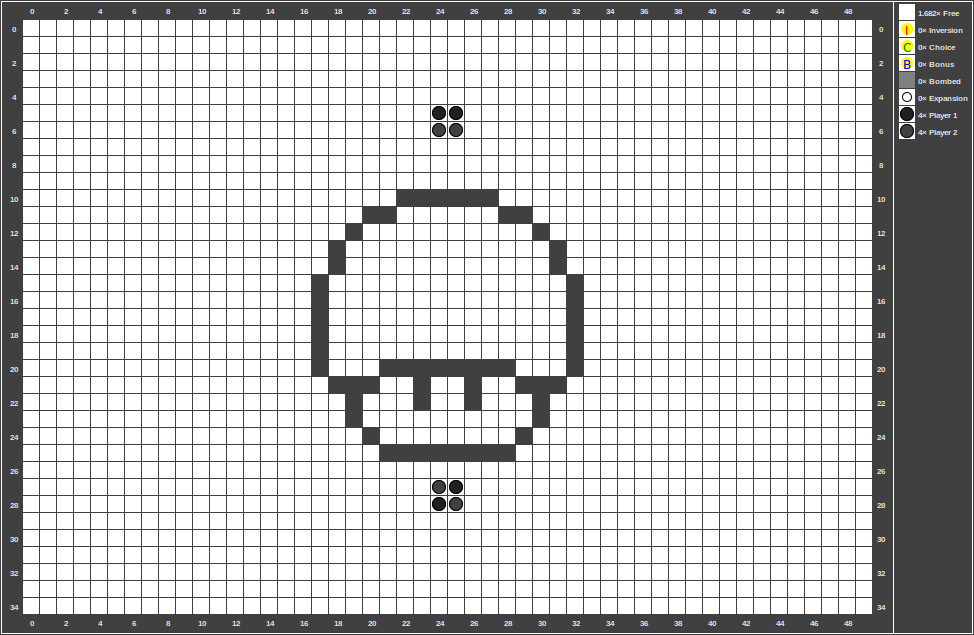
\includegraphics[width=0.5\linewidth]{pics/gamefield01.png}
	\captionof{figure}[Spielfeld 01]{Unbespieltes Spielfeld}
	\label{fig:reversi01}
\end{minipage}


Nachdem das Spielt gestartet wurde und beide Spielphasen durchlaufen wurden, siegt schließlich der Spieler mit der Farbe rot.

\vspace{1em}
\begin{minipage}{\linewidth}
	\centering
	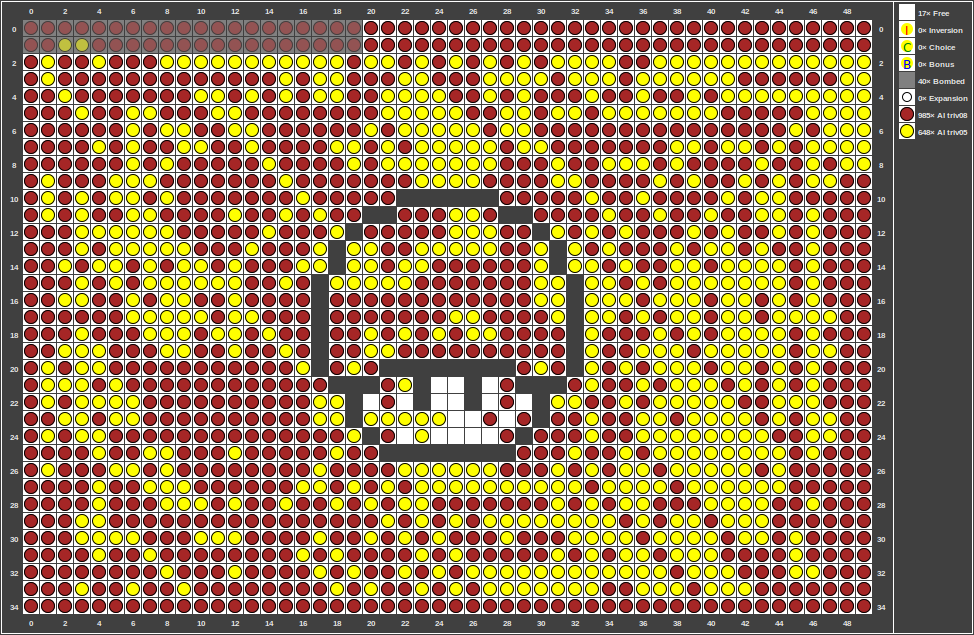
\includegraphics[width=0.5\linewidth]{pics/gamefield02.png}
	\captionof{figure}[Spielfeld 02]{Finales Spielfeld}
	\label{fig:reversi2}
\end{minipage}


\subsection{Tabellen}
In diesem Abschnitt wird eine Tabelle (siehe Tabelle \ref{tab:beispiel}) dargestellt.

\vspace{1em}
\begin{table}[!h]
	\centering
	\begin{tabular}{|l|l|l|}
		\hline
		\textbf{Name} & \textbf{Name} & \textbf{Name}\\
		\hline
		1 & 2 & 3\\
		\hline
		4 & 5 & 6\\
		\hline
		7 & 8 & 9\\
		\hline
	\end{tabular}
	\caption{Beispieltabelle}
	\label{tab:beispiel}
\end{table}


\subsection{Auflistung}
Für Auflistungen wird die \texttt{enumerate}- oder \texttt{itemize}-Umgebung genutzt.

\begin{itemize}
	\item Nur
	\item ein
	\item Beispiel.
\end{itemize}

\subsection{Listings}
Sehen Sie in Listing \ref{lst:helloworld} ein Beispiel für das Einbinden von Quellcode mit Syntax-Highlighting.

\vspace{1em}
%\lstinputlisting[caption=Brute Force-Ansatz für das MaxTeilsum2D-Problem, label=lst:maxTeilsumZweiD,basicstyle=\ttfamily\scriptsize]{code/maxTeilsum2DBruteForce.txt}
\lstinputlisting[caption=Hello World Program, label=lst:helloworld,basicstyle=\ttfamily\scriptsize]{code/helloworld.c}

\subsection{Gleichungen}
Formatierung von Formeln:
\begin{itemize}
  \item Formelzeichen sind in kursiv zu setzen
  \item Zahlen, Einheiten und Funktionsnamen sind in normaler Schriftart zu setzen (nicht kursiv)
  \item Häufig wird fälschlicherweise das Symbol * als Multiplikationszeichen verwendet
  \item Zwischen Zahl und Einheit ist ein Leerzeichen zu setzen
\end{itemize}

Frequency Modulation (FM) is a wireless transmission system patent-registered by Edwin H. Armstrong in 1933. It is still widespread in the area of audio broadcasting today. In case of the frequency modulation the amplitude of the desired message signal varies the frequency (the argument) of the sinusoidal carrier. The general FM oscillation is formulated with 
\begin{equation}
u_{\textrm{FM}}(t)= a_0 \cos(\Psi(t)+\varphi_0) 
\label{eqn:fmosc}
\end{equation}

To simplify matters, only an one-tone modulation signal is considered to characterize the spectrum of FM-signals at first
\begin{multline}
u_{\textrm{FM}}(t)=\hat u_T \cdot [J_0(\eta)\cos\omega_Tt + \sum_{n=1}^{+\infty} J_n(\eta) \cdot (\cos[(\omega_T+n\omega_1)t]+(-1)^n \cos[(\omega_T-n\omega_1)t])] 
\\ \ \mbox{with Bessel functions:} \ J_n(\eta)= \frac{(-1)^n}{\pi} \int_0^{\pi} e^{j\eta\sin x} \cdot \cos(nx) dx 
\end{multline}

\subsection{Verwendung von Abkürzungen}
Die Abkürzungen können so verwendet werden:
Beim ersten Mal der Verwendung (vgl. Einleitung) wird die Abkürzung ausgeschrieben \ac{BA}. Beim zweiten Mal oder folgenden Malen wird nur noch die Abkürzung verwendet \ac{BA}.
Aber setzen Sie Abkürzungen sparsam ein.

\subsection{Tipps}
Die Quellen befinden sich in der Datei \textit{quellen.bib}. 
Alle Literaturangaben müssen im Text referenziert werden. Die höchstwertigen Quellen stellen dabei Zeitschriftenartikel \cite{Laprie2004}, gefolgt von Konferenzbeiträgen \cite{Agrou2011}, Patenten \cite{Grisenthwaite2012}, Standards \cite{ARINC2005}, Fachbüchern \cite{Kopetz2011},  Datenblättern \cite{Freescale2015}, Techreports und White-Papern \cite{Aswadhati2011} und zuletzt Onlinequellen \cite{Xil2010} dar.

\pagebreak



% ----------------------------------------------------------------------------------------------------------
% Anhang
% ----------------------------------------------------------------------------------------------------------
\pagenumbering{Roman}
\setcounter{page}{1}
\lhead{Anhang \thesection}

\begin{appendix}
\section*{Anhang}
\phantomsection
\addcontentsline{toc}{section}{Anhang}
\addtocontents{toc}{\vspace{-0.5em}}

\section{Domändenmodell}
Ein toller Anhang.

\subsection*{Screenshot}
\label{app:screenshot}
Unterkategorie, die nicht im Inhaltsverzeichnis auftaucht.
\pagebreak

\end{appendix}
\pagebreak

% ----------------------------------------------------------------------------------------------------------
% Abkürzungsverzeichnis
% ----------------------------------------------------------------------------------------------------------
\addsec{Abkürzungsverzeichnis}
\begin{acronym}[KDE]
	\acro{BA}[BA]{Bachelorarbeit}
	\acro{MA}[MA]{Masterarbeit}
\end{acronym}
\pagebreak


% ----------------------------------------------------------------------------------------------------------
% Abbildungsverzeichnis (optional)
% ----------------------------------------------------------------------------------------------------------
%\listoffigures
%\pagebreak

% ----------------------------------------------------------------------------------------------------------
% Tabellenverzeichnis (optional)
% ----------------------------------------------------------------------------------------------------------
%\listoftables
%\pagebreak

% ----------------------------------------------------------------------------------------------------------
% Listingsverzeichnis (optional; Code nur, wenn wirklich sinnvoll und wichtig)
% ----------------------------------------------------------------------------------------------------------
%\lstlistoflistings
%\pagebreak

% ----------------------------------------------------------------------------------------------------------
% Eidestattliche Erklärung
% ----------------------------------------------------------------------------------------------------------
%\addsec{Eidesstattliche Erklärung}
%...
%\pagebreak

% ----------------------------------------------------------------------------------------------------------
% Literatur
% ----------------------------------------------------------------------------------------------------------
\renewcommand\refname{Literaturverzeichnis}
\lhead{}
%\bibliographystyle{alpha}
\bibliographystyle{ieeetr}
\bibliography{quellen}
\pagebreak

% ----------------------------------------------------------------------------------------------------------
% Inhalt des Datenträgers
% ----------------------------------------------------------------------------------------------------------
\addsec{Inhalt des Datenträgers}
\begin{itemize}
	\item $\ldots$
	\item $\ldots$
\end{itemize}
\pagebreak

\end{document}
